\chapter{Introductie}

\noindent Met deze reader verkrijgt de lezer een stevige fundatie voor het gebruik van ROS 2 aan de hand van concrete codevoorbeelden. ROS is een open source software framework en komt met veel tools voor het programmeren, het compilen van code, het testen en het simuleren van hardware. Een belangrijke eigenschap van ROS is dat het de communicatie verzorgt tussen de verschillende processen (``robot onderdelen''). ROS maakt het hiermee mogelijk software te schrijven voor \'e\'en onderdeel zonder dat men zich zorgen hoeft te maken over elk klein detail van de andere onderdelen. De flexibiliteit en herbruikbaarheid van code en hardware wordt hiermee vergroot. Een in ROS geprogrammeerde ultra-sound sensor kan zowel werken op de Care-O-Bot 4 als op de Terminator\footnote{De aanname is dat Arnold Schwarzenegger draait met ROS (\url{https://www.imdb.com/title/tt0088247/}).}. Het is dan ook niet gek dat de meeste robot(onderdelen)fabrikanten software leveren die werkt met ROS. Hiermee kan hun hardware flexibel worden gebruikt in de meest uiteenlopende projecten. Daarnaast zorgt de open-source-community van ROS dat vele libraries beschikbaar zijn.

\begin{figure}[ht]
\begin{center}
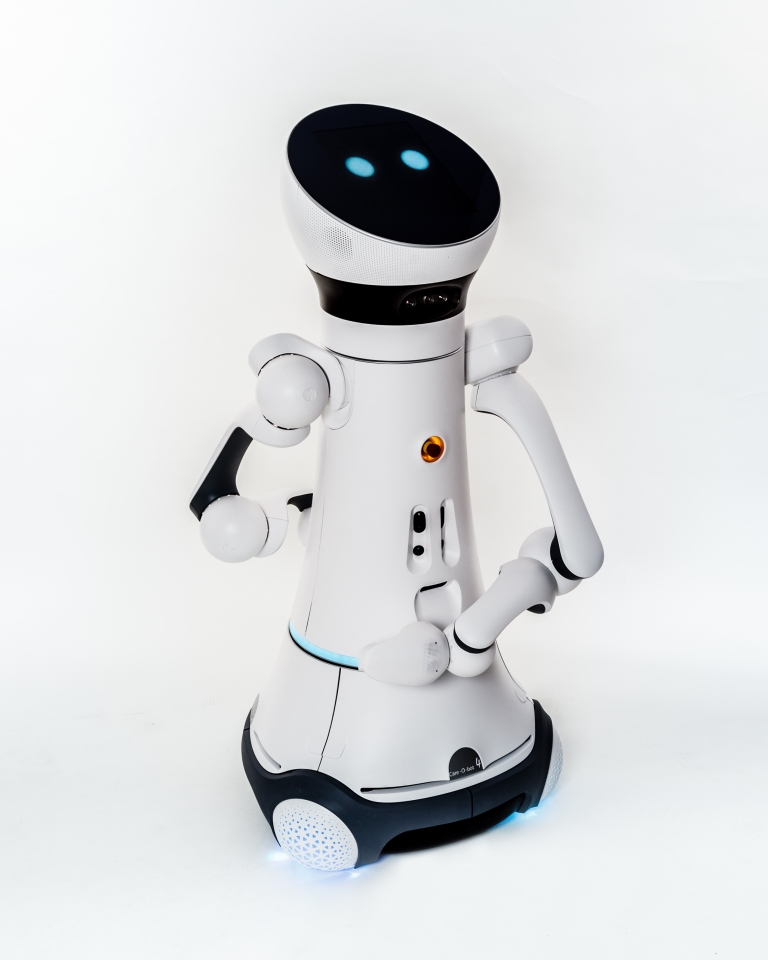
\includegraphics[scale=0.15]{Care-O-bot_4}\\
\end{center}
\caption{De zorgrobot Care-O-bot 4\\\tiny{(Foto door Fraunhofer IPA)}}\label{fig:care-o-bot4}
\end{figure}

De voordelen van ROS zijn zichtbaar bij de zorgrobot Care-O-Bot 4 (zie figuur \ref{fig:care-o-bot4}). Deze heeft verschillende sensoren (microfoon, knoppen, camera's, LiDar) en meerdere actuatoren (wielen, robotarmen, scherm, etc.) die met elkaar moeten samenwerken en communiceren. Elke sensor en actuator heeft zijn eigen (programmeer)uitdagingen die we graag, voor zo ver mogelijk, per onderdeel aanpakken. Verder willen we graag flexibel zijn in welke sensoren en actuatoren de Care-O-Bot gebruikt. ROS helpt ons hierbij. Het doel van ROS is het verzorgen van een standaard voor robot software development dat resulteert in software dat werkt op elke robot. 

De reader start bij de basis, een simpele ROS-node, en gaat vervolgens in op de drie manieren van communicatie in ROS 2. Naast de codevoorbeelden in de reader is zijn er nog meer codevoorbeelden beschikbaar op de git. Voordat men zijn/haar eigen code met ROS gaat schrijven raden wij sterk aan of hoofdstuk 2 en 3 van deze reader te lezen en de stappen van appendix \ref{chp:HelloNode_package} te doorlopen.\\

Deze reader is ontwikkeld ter ondersteuning van de cursus \textit{World} van de Hogeschool Arnhem en Nijmegen. De reader bevat de belangrijkste functionaliteiten van ROS 2, maar heeft een focus op de C++code. Meer informatie over ROS 2 kan men vinden in de documentatie van ROS 2:
\begin{center}
    \url{https://docs.ros.org/en/foxy/}
\end{center}

Voordat de lezer vol enthousiasme de reader in duikt raden wij aan om eerst ROS 2 te installeren. 

\section{Installatie en gebruik}
Voor de installatie van ROS verwijzen we naar de tutorial van ROS. De auteur heeft gebruik gemaakt van ROS 2 Foxy Fitzroy op Linux.
\begin{center}
    \url{https://docs.ros.org/en/foxy/Installation.html}
\end{center}

\noindent 

\noindent Met ROS 2 maken we gebruik van de library \textit{rclcpp}. De documentatie hiervan is te vinden op:
\begin{center}
    \url{http://docs.ros2.org/latest/api/rclcpp/}
\end{center}

\vspace{1cm}
